% !TeX program = xelatex
\documentclass[
  convert={density=500, size=600, outext=.png}, 
  border=2pt
]{standalone}

\usepackage{fontspec}
\defaultfontfeatures{Ligatures={NoCommon,%
			NoDiscretionary,%
			NoHistoric,%
			NoRequired,%
			NoContextual}}
\setsansfont{Carlito}[%
	SmallCapsFeatures={Letters=SmallCaps},%
	SmallCapsFont={Roboto},%
	ItalicFeatures={SmallCapsFont=Roboto-Italic},%
	BoldFeatures={SmallCapsFont=Roboto-Bold},%
	BoldItalicFeatures={SmallCapsFont=Roboto-BoldItalic}%
]

\usepackage{tikz}
\usepackage{tikz-cd}
\usetikzlibrary{%
	calc,%
	arrows.meta,%
	arrows,%
	automata,%
	overlay-beamer-styles,%
	snakes,%
	shapes.arrows,%
	shapes.geometric,%
	shapes.symbols,%
	fit,%
	positioning,%
	decorations.pathreplacing,%
	backgrounds,%
}
\tikzset{
	>=Triangle,%
	nodes={align=center},%
	comp/.style={%
			draw,%
			rectangle,%
			very thick,%
			rounded corners,%
			minimum width=2.5cm,%
			minimum height=1cm,%
			fill=white},%
	input/.style={draw,%
			rectangle,%
			thick,%
			minimum width=2.5cm,%
			minimum height=1cm,%
			fill=white},%
	classnode/.style={%
			fill=cgreenlight,%
			rectangle,%
			draw,%
			inner xsep=0},%
	interfacenode/.style={%
			fill=corangelight,%
			rectangle,%
			draw,%
			inner xsep=0},%
	abstractclassnode/.style={%
			fill=cbluelight,%
			rectangle,%
			draw,%
			inner xsep=0},%
	inlinenode/.style={%
			inner xsep=.5cm,%
			minimum height=.6cm},%
}

\definecolor{reddy}{RGB}{172, 0, 51}
\definecolor{dkred}{rgb}{.6, 0, 0}
\definecolor{dkgreen}{rgb}{0, .5, 0}
\definecolor{dkblue}{rgb}{0, 0, .5}
\definecolor{cred}{RGB}{219, 68, 55}
\definecolor{credlight}{RGB}{250, 227, 225}
\definecolor{cgreen}{RGB}{3, 148, 77}
\definecolor{cgreenlight}{RGB}{209, 251, 230}
\definecolor{cblue}{RGB}{2, 119, 189}
\definecolor{cbluelight}{RGB}{208, 237, 254}
\definecolor{corange}{RGB}{173, 128, 2}
\definecolor{corangelight}{RGB}{253, 219, 123}
\newcommand{\cblue}[1]{\textcolor{cblue}{#1}}
\newcommand{\bfcblue}[1]{\textcolor{cblue}{\textbf{#1}}}
\newcommand{\cred}[1]{\textcolor{cred}{#1}}
\newcommand{\bfcred}[1]{\textcolor{cred}{\textbf{#1}}}
\newcommand{\cgreen}[1]{\textcolor{cgreen}{#1}}
\newcommand{\bfcgreen}[1]{\textcolor{cgreen}{\textbf{#1}}}
\newcommand{\corange}[1]{\textcolor{corange}{#1}}
\newcommand{\bfcorange}[1]{\textcolor{corange}{\textbf{#1}}}
\newcommand{\interfacename}[1]{\underline{\textbf{\textit{#1}}}}
\newcommand{\absclassname}[1]{\textbf{\textit{#1}}}
\newcommand{\classname}[1]{\textbf{#1}}

\usepackage{amsmath}
\usepackage{amsfonts}
\usepackage{amssymb}

\usepackage{silence}
\WarningsOff*


\begin{document}
\sffamily

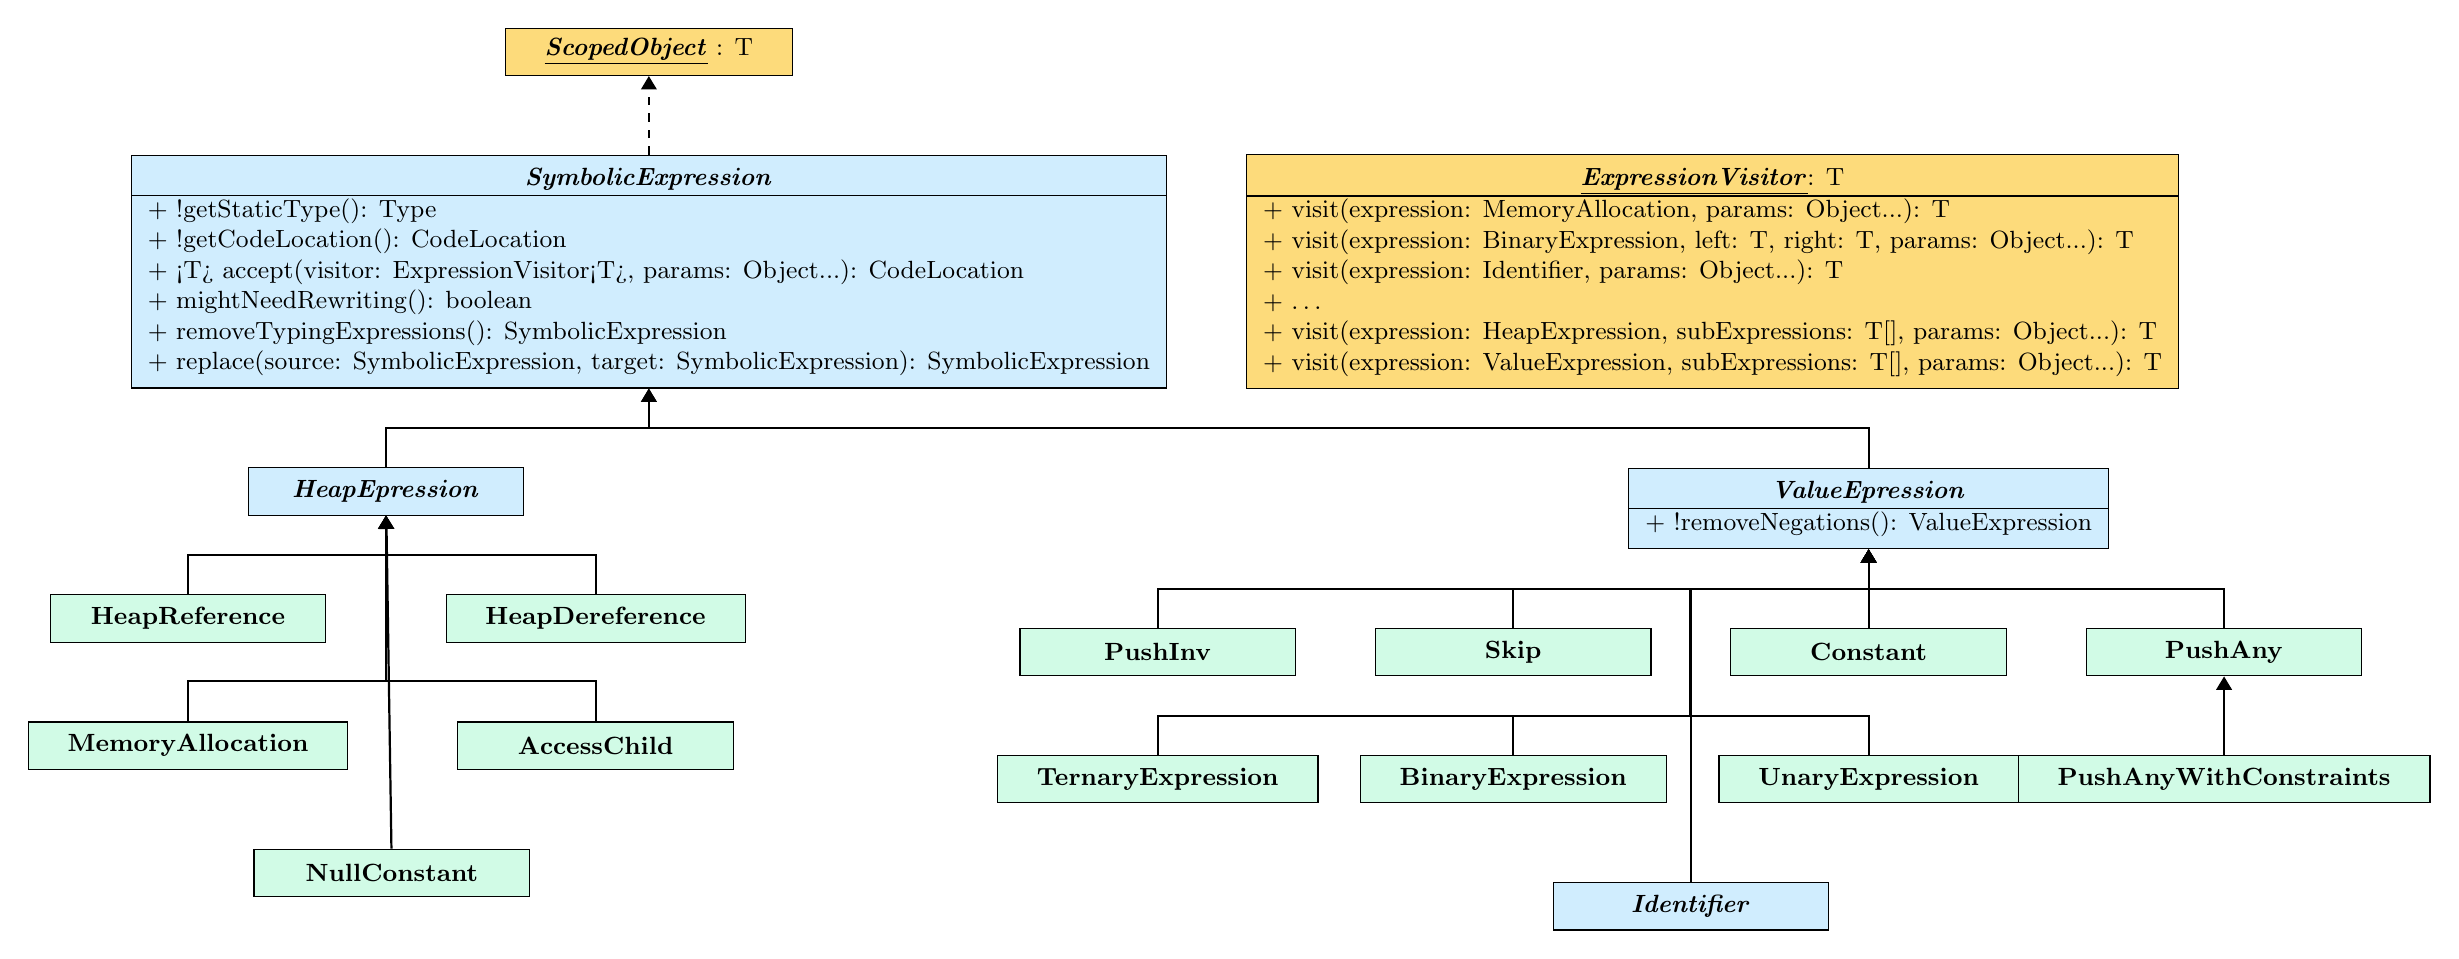
\begin{tikzpicture}[nodes={font={\small}, minimum width=3.5cm}]%
	\node[interfacenode, inlinenode] (so) {\interfacename{ScopedObject} : T};

	\node[abstractclassnode] (se) [below=of so] {\begin{tabular}{l}
			\multicolumn{1}{c}{\absclassname{SymbolicExpression}}                                 \\
			\hline
			+ !getStaticType(): Type                                                              \\
			+ !getCodeLocation(): CodeLocation                                                    \\
			+ <T> accept(visitor: ExpressionVisitor<T>, params: Object...): CodeLocation          \\
			+ mightNeedRewriting(): boolean                                                       \\
			+ removeTypingExpressions(): SymbolicExpression                                       \\
			+ replace(source: SymbolicExpression, target: SymbolicExpression): SymbolicExpression \\
		\end{tabular}};

	\node[interfacenode] (ev) [right=of se] {\begin{tabular}{l}
			\multicolumn{1}{c}{\interfacename{ExpressionVisitor}: T}                        \\
			\hline
			+ visit(expression: MemoryAllocation, params: Object...): T                     \\
			+ visit(expression: BinaryExpression, left: T, right: T, params: Object...): T  \\
			+ visit(expression: Identifier, params: Object...): T                           \\
			+ $\dots$                                                                       \\
			+ visit(expression: HeapExpression, subExpressions: T[], params: Object...): T  \\
			+ visit(expression: ValueExpression, subExpressions: T[], params: Object...): T \\
		\end{tabular}};

	\node[abstractclassnode, inlinenode] (he) [below left=1cm and -5cm of se] {\absclassname{HeapEpression}};
	\node[classnode, inlinenode] (hr) [below left=1cm and -1cm of he] {\classname{HeapReference}};
	\node[classnode, inlinenode] (hd) [below right=1cm and -1cm of he] {\classname{HeapDereference}};
	\node[classnode, inlinenode] (ma) [below=of hr] {\classname{MemoryAllocation}};
	\node[classnode, inlinenode] (ac) [below=of hd] {\classname{AccessChild}};
	\node[classnode, inlinenode] (nc) [below=of $(ma.south)!0.5!(ac.south)$] {\classname{NullConstant}};



	\node[abstractclassnode] (ve) [below right=1cm and -7cm of ev] {\begin{tabular}{l}
			\multicolumn{1}{c}{\absclassname{ValueEpression}} \\
			\hline
			+ !removeNegations(): ValueExpression             \\
		\end{tabular}};
	\node[classnode, inlinenode] (const) [below=of ve] {\classname{Constant}};
	\node[classnode, inlinenode] (skip) [left=of const] {\classname{Skip}};
	\node[classnode, inlinenode] (pi) [left=of skip] {\classname{PushInv}};
	\node[classnode, inlinenode] (pa) [right=of const] {\classname{PushAny}};
	\node[classnode, inlinenode] (pac) [below=of pa] {\classname{PushAnyWithConstraints}};
	\node[classnode, inlinenode] (ue) [below=of const] {\classname{UnaryExpression}};
	\node[classnode, inlinenode] (be) [below=of skip] {\classname{BinaryExpression}};
	\node[classnode, inlinenode] (te) [below=of pi] {\classname{TernaryExpression}};
	\node[abstractclassnode, inlinenode] (id) [below=of $(be.south)!0.5!(ue.south)$] {\absclassname{Identifier}};

	\draw[->, thick, dashed] (se) to (so);
	\draw[->, thick] (he) |- ($(se.south)+(0,-0.5)$) to (se);
	\draw[->, thick] (ve) |- ($(se.south)+(0,-0.5)$) to (se);
	\draw[->, thick] (nc) to (he);
	\draw[->, thick] (ma) |- ($(he.south)+(0,-2.1)$) to (he);
	\draw[->, thick] (ac) |- ($(he.south)+(0,-2.1)$) to (he);
	\draw[->, thick] (hr) |- ($(he.south)+(0,-0.5)$) to (he);
	\draw[->, thick] (hd) |- ($(he.south)+(0,-0.5)$) to (he);
	\draw[->, thick] (const) to (ve);
	\draw[->, thick] (skip) |- ($(ve.south)+(0,-0.5)$) to (ve);
	\draw[->, thick] (pa) |- ($(ve.south)+(0,-0.5)$) to (ve);
	\draw[->, thick] (pac) to (pa);
	\draw[->, thick] (pi) |- ($(ve.south)+(0,-0.5)$) to (ve);
	\draw[->, thick] (id) |- ($(ve.south)+(0,-0.5)$) to (ve);
	\draw[->, thick] (be) |- ($(be.north)+(2.25,0.5)$) |- ($(ve.south)+(0,-0.5)$) to (ve);
	\draw[->, thick] (te) |- ($(be.north)+(2.25,0.5)$) |- ($(ve.south)+(0,-0.5)$) to (ve);
	\draw[->, thick] (ue) |- ($(be.north)+(2.25,0.5)$) |- ($(ve.south)+(0,-0.5)$) to (ve);
\end{tikzpicture}

\end{document}
